% =====================================================================
% 06_bicubic_example.tex -- Worked Example: Bicubic Bezier Surface
% Compute S(0.5, 0.5) on a 4x4 control net step-by-step.
% Bilingual EN | VI cheatsheet section for IT516 Advanced Computer Graphics
% =====================================================================

\begin{paracol}{2}

% =====================================================================
% ENGLISH COLUMN
% =====================================================================
\section*{6.\ Worked Example: Bicubic Bezier Surface (4$\times$4) at $(u,v)=(0.5,0.5)$}

\subsection*{6.1 Setup --- the 4$\times$4 Control Net}

A \textbf{bicubic Bezier surface} (degree 3 in both $u$ and $v$) needs a $4\times 4$ control net $\{P_{ij}\}_{i,j=0}^{3}$. We use the following ``hill / tent'' net (rows $i$ run along $u$, columns $j$ run along $v$):
\[
\renewcommand{\arraystretch}{1.1}
\begin{array}{c|cccc}
 & j=0 & j=1 & j=2 & j=3 \\\hline
i{=}0 & (0,0,0) & (1,0,1) & (2,0,1) & (3,0,0) \\
i{=}1 & (0,1,1) & (1,1,3) & (2,1,3) & (3,1,1) \\
i{=}2 & (0,2,1) & (1,2,3) & (2,2,3) & (3,2,1) \\
i{=}3 & (0,3,0) & (1,3,1) & (2,3,1) & (3,3,0)
\end{array}
\]
The $(x,y)$ are on the integer grid; only the $z$-component varies (saddle/tent peak in the centre). We want $S(0.5,\,0.5)$.

The surface formula:
\[
S(u,v)=\sum_{i=0}^{3}\sum_{j=0}^{3} B_i^3(u)\,B_j^3(v)\,P_{ij}.
\]
We will compute $S(0.5,0.5)$ \textbf{three ways} and check they match.

% ---------------------------------------------------------------------
\subsection*{6.2 Method 1 --- Row-first De Casteljau}

\textbf{Step A.} For each row $i$, run De Casteljau in $v$ at $v=0.5$ on the four points $P_{i0},P_{i1},P_{i2},P_{i3}$ to obtain $Q_i$.

\textbf{Row 0:} $(0,0,0),(1,0,1),(2,0,1),(3,0,0)$
\begin{align*}
\text{L1: }& \tfrac{1}{2}(P_{00}{+}P_{01})=(0.5,0,0.5)\\
           & \tfrac{1}{2}(P_{01}{+}P_{02})=(1.5,0,1)\\
           & \tfrac{1}{2}(P_{02}{+}P_{03})=(2.5,0,0.5)\\
\text{L2: }& \tfrac{1}{2}((0.5,0,0.5){+}(1.5,0,1))=(1.0,0,0.75)\\
           & \tfrac{1}{2}((1.5,0,1){+}(2.5,0,0.5))=(2.0,0,0.75)\\
\text{L3: }& Q_0=\tfrac{1}{2}((1.0,0,0.75){+}(2.0,0,0.75))\\
           &\phantom{Q_0}=(1.5,\,0,\,0.75)
\end{align*}

\textbf{Row 1:} $(0,1,1),(1,1,3),(2,1,3),(3,1,1)$
\begin{align*}
\text{L1: }& (0.5,1,2),\;(1.5,1,3),\;(2.5,1,2)\\
\text{L2: }& (1.0,1,2.5),\;(2.0,1,2.5)\\
\text{L3: }& Q_1=(1.5,\,1,\,2.5)
\end{align*}

\textbf{Row 2:} same $z$-pattern as Row 1 (only $y$ changes from 1 to 2), so by the affine-invariance of De Casteljau the result is
\[
Q_2=(1.5,\,2,\,2.5).
\]

\textbf{Row 3:} same $z$-pattern as Row 0, so
\[
Q_3=(1.5,\,3,\,0.75).
\]

\textbf{Step B.} Now run De Casteljau in $u$ at $u=0.5$ on $Q_0,Q_1,Q_2,Q_3$:
\begin{align*}
\text{L1: }& \tfrac{1}{2}(Q_0{+}Q_1)=(1.5,\,0.5,\,1.625)\\
           & \tfrac{1}{2}(Q_1{+}Q_2)=(1.5,\,1.5,\,2.5)\\
           & \tfrac{1}{2}(Q_2{+}Q_3)=(1.5,\,2.5,\,1.625)\\
\text{L2: }& \tfrac{1}{2}((1.5,0.5,1.625){+}(1.5,1.5,2.5))\\
           &\quad =(1.5,\,1.0,\,2.0625)\\
           & \tfrac{1}{2}((1.5,1.5,2.5){+}(1.5,2.5,1.625))\\
           &\quad =(1.5,\,2.0,\,2.0625)\\
\text{L3: }& S(0.5,0.5)=\tfrac{1}{2}((1.5,1.0,2.0625){+}(1.5,2.0,2.0625))
\end{align*}
\[
\boxed{\,S(0.5,\,0.5)=(1.5,\;1.5,\;2.0625)\,}
\]

% ---------------------------------------------------------------------
\subsection*{6.3 Method 2 --- Column-first verification}

Swap the order: first De Casteljau in $u$ on each column $j$ at $u=0.5$ to obtain $R_j$, then in $v$ on $R_0,R_1,R_2,R_3$ at $v=0.5$.

\textbf{Column 0:} $(0,0,0),(0,1,1),(0,2,1),(0,3,0)$\\
$\Rightarrow R_0=(0,\,1.5,\,0.75)$ (same $z$-arithmetic as Row 0).

\textbf{Column 1:} $(1,0,1),(1,1,3),(1,2,3),(1,3,1)$\\
$\Rightarrow R_1=(1,\,1.5,\,2.5)$.

\textbf{Column 2:} by symmetry $R_2=(2,\,1.5,\,2.5)$.

\textbf{Column 3:} by symmetry $R_3=(3,\,1.5,\,0.75)$.

Now De Casteljau on $R_0,\dots,R_3$ at $v=0.5$:
\begin{align*}
\text{L1: }& (0.5,1.5,1.625),\;(1.5,1.5,2.5),\;(2.5,1.5,1.625)\\
\text{L2: }& (1.0,1.5,2.0625),\;(2.0,1.5,2.0625)\\
\text{L3: }& (1.5,\,1.5,\,2.0625)\quad\checkmark
\end{align*}
Same answer --- the tensor-product structure makes the two orders commute.

% ---------------------------------------------------------------------
\subsection*{6.4 Method 3 --- Direct Bernstein verification}

At $t=0.5$ the cubic Bernstein basis is
\[
B_i^3(0.5)=\tfrac{1}{8}\big(1,\,3,\,3,\,1\big),\quad i=0,1,2,3.
\]
The bicubic weights $w_{ij}=B_i^3(0.5)\,B_j^3(0.5)$ form (in units of $1/64$):
\[
[w_{ij}]\cdot 64=
\begin{pmatrix}
1 & 3 & 3 & 1\\
3 & 9 & 9 & 3\\
3 & 9 & 9 & 3\\
1 & 3 & 3 & 1
\end{pmatrix}.
\]
Sum check: $4(1)+8(3)+4(9)=4{+}24{+}36=64$. \checkmark

\textbf{Compute $z$-component first} (the only non-trivial one). Z-matrix is
\[
[z_{ij}]=\begin{pmatrix}0&1&1&0\\1&3&3&1\\1&3&3&1\\0&1&1&0\end{pmatrix}.
\]
\begin{align*}
64\,z &= \underbrace{1\!\cdot\!0\!\cdot\!4}_{\text{corners}} + \underbrace{3\!\cdot\!1\!\cdot\!8}_{\text{edge mids}} + \underbrace{9\!\cdot\!3\!\cdot\!4}_{\text{interior}}\\
&= 0 + 24 + 108 = 132,\\
z &= 132/64 = 2.0625.\;\checkmark
\end{align*}

\textbf{$x$-component:} by row sums, $\sum_j w_{ij}x_{ij}$ uses $x_{ij}=j$, weighted along each row by $(1,3,3,1)/8$:
\[
\bar{x}_{\text{row}} = \tfrac{1\cdot0+3\cdot1+3\cdot2+1\cdot3}{8}=\tfrac{12}{8}=1.5,
\]
and this is the same for every row, so $x=1.5$.

\textbf{$y$-component:} symmetric argument with $y_{ij}=i$ gives $y=1.5$.

Final result $(1.5,1.5,2.0625)$ \emph{matches the De Casteljau answer.} \checkmark

% ---------------------------------------------------------------------
\subsection*{6.5 Control Net Diagram}

\begin{center}
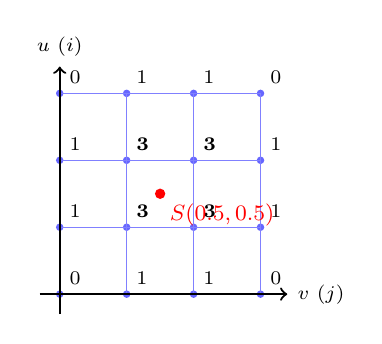
\begin{tikzpicture}[scale=0.85,every node/.style={font=\scriptsize}]
  % grid
  \foreach \i in {0,1,2,3}{
    \foreach \j in {0,1,2,3}{
      \fill[blue!60] (\j,\i) circle (1.6pt);
    }
  }
  % row/col polylines
  \foreach \i in {0,1,2,3}{
    \draw[blue!50,thin] (0,\i)--(1,\i)--(2,\i)--(3,\i);
  }
  \foreach \j in {0,1,2,3}{
    \draw[blue!50,thin] (\j,0)--(\j,1)--(\j,2)--(\j,3);
  }
  % z-labels
  \node[above right] at (0,0) {$0$};
  \node[above right] at (1,0) {$1$};
  \node[above right] at (2,0) {$1$};
  \node[above right] at (3,0) {$0$};
  \node[above right] at (0,1) {$1$};
  \node[above right] at (1,1) {$\mathbf{3}$};
  \node[above right] at (2,1) {$\mathbf{3}$};
  \node[above right] at (3,1) {$1$};
  \node[above right] at (0,2) {$1$};
  \node[above right] at (1,2) {$\mathbf{3}$};
  \node[above right] at (2,2) {$\mathbf{3}$};
  \node[above right] at (3,2) {$1$};
  \node[above right] at (0,3) {$0$};
  \node[above right] at (1,3) {$1$};
  \node[above right] at (2,3) {$1$};
  \node[above right] at (3,3) {$0$};
  % evaluation point S(0.5,0.5)
  \fill[red] (1.5,1.5) circle (2.2pt);
  \node[red,below right] at (1.5,1.5) {\footnotesize $S(0.5,0.5)$};
  % axes
  \draw[->,thick] (-0.3,0)--(3.4,0) node[right]{$v$ ($j$)};
  \draw[->,thick] (0,-0.3)--(0,3.4) node[above]{$u$ ($i$)};
\end{tikzpicture}
\end{center}
\textit{Top-down view: numbers are $z$-heights of $P_{ij}$. Red dot = projected evaluation point.}

% ---------------------------------------------------------------------
\subsection*{6.6 Exam Tips}

\begin{itemize}[leftmargin=*,nosep]
  \item \textbf{Direction discipline:} write down which axis is $u$ (rows $i$) and which is $v$ (columns $j$) before the first arithmetic step.
  \item \textbf{Row-first is usually faster} on paper: you can reuse symmetry between rows (e.g.\ Row 0 vs Row 3, Row 1 vs Row 2) to skip duplicate work.
  \item \textbf{Always sanity-check with Bernstein.} At $(0.5,0.5)$ the cubic weights are $(1,3,3,1)/8$, so the $4\times4$ weights are $\{1,3,9\}/64$ --- \emph{memorise these}.
  \item Check the corner/edge/interior tally: $4{\cdot}1+8{\cdot}3+4{\cdot}9=64$.
  \item For other $(u,v)$, compute $B_i^3(u)$ and $B_j^3(v)$ separately, then form the outer product.
  \item $S(u,v)$ at the corners equals the corner control points: $S(0,0)=P_{00}$ etc.\ --- handy for instant validation.
\end{itemize}

% =====================================================================
\switchcolumn
% =====================================================================
% VIETNAMESE COLUMN
% =====================================================================
\section*{6.\ Ví dụ tính tay: Mặt Bezier bicubic (4$\times$4) tại $(u,v)=(0.5,0.5)$}

\subsection*{6.1 Thiết lập --- lưới control net 4$\times$4}

Một \textbf{mặt Bezier bicubic} (bậc 3 theo cả $u$ và $v$) cần lưới $4\times 4$ control point $\{P_{ij}\}_{i,j=0}^{3}$. Ta dùng lưới ``đồi/lều'' sau (hàng $i$ chạy theo hướng $u$, cột $j$ chạy theo hướng $v$):
\[
\renewcommand{\arraystretch}{1.1}
\begin{array}{c|cccc}
 & j=0 & j=1 & j=2 & j=3 \\\hline
i{=}0 & (0,0,0) & (1,0,1) & (2,0,1) & (3,0,0) \\
i{=}1 & (0,1,1) & (1,1,3) & (2,1,3) & (3,1,1) \\
i{=}2 & (0,2,1) & (1,2,3) & (2,2,3) & (3,2,1) \\
i{=}3 & (0,3,0) & (1,3,1) & (2,3,1) & (3,3,0)
\end{array}
\]
Toạ độ $(x,y)$ nằm trên lưới số nguyên; chỉ thành phần $z$ thay đổi (tạo dạng yên ngựa/đỉnh đồi ở giữa). Ta cần tính $S(0.5,\,0.5)$.

Công thức mặt:
\[
S(u,v)=\sum_{i=0}^{3}\sum_{j=0}^{3} B_i^3(u)\,B_j^3(v)\,P_{ij}.
\]
Ta sẽ tính $S(0.5,0.5)$ \textbf{theo ba cách} và kiểm tra trùng kết quả.

% ---------------------------------------------------------------------
\subsection*{6.2 Cách 1 --- De Casteljau theo hàng trước}

\textbf{Bước A.} Với mỗi hàng $i$, chạy De Casteljau theo $v$ tại $v=0.5$ trên 4 điểm $P_{i0},P_{i1},P_{i2},P_{i3}$ để được $Q_i$.

\textbf{Hàng 0:} $(0,0,0),(1,0,1),(2,0,1),(3,0,0)$
\begin{align*}
\text{L1: }& \tfrac{1}{2}(P_{00}{+}P_{01})=(0.5,0,0.5)\\
           & \tfrac{1}{2}(P_{01}{+}P_{02})=(1.5,0,1)\\
           & \tfrac{1}{2}(P_{02}{+}P_{03})=(2.5,0,0.5)\\
\text{L2: }& \tfrac{1}{2}((0.5,0,0.5){+}(1.5,0,1))=(1.0,0,0.75)\\
           & \tfrac{1}{2}((1.5,0,1){+}(2.5,0,0.5))=(2.0,0,0.75)\\
\text{L3: }& Q_0=\tfrac{1}{2}((1.0,0,0.75){+}(2.0,0,0.75))\\
           &\phantom{Q_0}=(1.5,\,0,\,0.75)
\end{align*}

\textbf{Hàng 1:} $(0,1,1),(1,1,3),(2,1,3),(3,1,1)$
\begin{align*}
\text{L1: }& (0.5,1,2),\;(1.5,1,3),\;(2.5,1,2)\\
\text{L2: }& (1.0,1,2.5),\;(2.0,1,2.5)\\
\text{L3: }& Q_1=(1.5,\,1,\,2.5)
\end{align*}

\textbf{Hàng 2:} có cùng pattern $z$ với Hàng 1 (chỉ $y$ đổi từ 1 sang 2), nhờ tính bất biến affine của De Casteljau ta có
\[
Q_2=(1.5,\,2,\,2.5).
\]

\textbf{Hàng 3:} có cùng pattern $z$ với Hàng 0, nên
\[
Q_3=(1.5,\,3,\,0.75).
\]

\textbf{Bước B.} Bây giờ chạy De Casteljau theo $u$ tại $u=0.5$ trên $Q_0,Q_1,Q_2,Q_3$:
\begin{align*}
\text{L1: }& \tfrac{1}{2}(Q_0{+}Q_1)=(1.5,\,0.5,\,1.625)\\
           & \tfrac{1}{2}(Q_1{+}Q_2)=(1.5,\,1.5,\,2.5)\\
           & \tfrac{1}{2}(Q_2{+}Q_3)=(1.5,\,2.5,\,1.625)\\
\text{L2: }& \tfrac{1}{2}((1.5,0.5,1.625){+}(1.5,1.5,2.5))\\
           &\quad =(1.5,\,1.0,\,2.0625)\\
           & \tfrac{1}{2}((1.5,1.5,2.5){+}(1.5,2.5,1.625))\\
           &\quad =(1.5,\,2.0,\,2.0625)\\
\text{L3: }& S(0.5,0.5)=\tfrac{1}{2}((1.5,1.0,2.0625){+}(1.5,2.0,2.0625))
\end{align*}
\[
\boxed{\,S(0.5,\,0.5)=(1.5,\;1.5,\;2.0625)\,}
\]

% ---------------------------------------------------------------------
\subsection*{6.3 Cách 2 --- Kiểm tra bằng cột trước}

Đảo thứ tự: De Casteljau theo $u$ trên mỗi cột $j$ tại $u=0.5$ để được $R_j$, rồi De Casteljau theo $v$ trên $R_0,R_1,R_2,R_3$ tại $v=0.5$.

\textbf{Cột 0:} $(0,0,0),(0,1,1),(0,2,1),(0,3,0)$\\
$\Rightarrow R_0=(0,\,1.5,\,0.75)$ ($z$ tính giống Hàng 0).

\textbf{Cột 1:} $(1,0,1),(1,1,3),(1,2,3),(1,3,1)$\\
$\Rightarrow R_1=(1,\,1.5,\,2.5)$.

\textbf{Cột 2:} đối xứng $R_2=(2,\,1.5,\,2.5)$.

\textbf{Cột 3:} đối xứng $R_3=(3,\,1.5,\,0.75)$.

De Casteljau trên $R_0,\dots,R_3$ tại $v=0.5$:
\begin{align*}
\text{L1: }& (0.5,1.5,1.625),\;(1.5,1.5,2.5),\;(2.5,1.5,1.625)\\
\text{L2: }& (1.0,1.5,2.0625),\;(2.0,1.5,2.0625)\\
\text{L3: }& (1.5,\,1.5,\,2.0625)\quad\checkmark
\end{align*}
Cùng kết quả --- cấu trúc tích tensor (tensor product) khiến hai thứ tự giao hoán.

% ---------------------------------------------------------------------
\subsection*{6.4 Cách 3 --- Kiểm tra trực tiếp bằng Bernstein}

Tại $t=0.5$ cơ sở Bernstein bậc 3 là
\[
B_i^3(0.5)=\tfrac{1}{8}\big(1,\,3,\,3,\,1\big),\quad i=0,1,2,3.
\]
Trọng số bicubic $w_{ij}=B_i^3(0.5)\,B_j^3(0.5)$ (đơn vị $1/64$):
\[
[w_{ij}]\cdot 64=
\begin{pmatrix}
1 & 3 & 3 & 1\\
3 & 9 & 9 & 3\\
3 & 9 & 9 & 3\\
1 & 3 & 3 & 1
\end{pmatrix}.
\]
Kiểm tra tổng: $4(1)+8(3)+4(9)=4{+}24{+}36=64$. \checkmark

\textbf{Tính thành phần $z$} (chỗ duy nhất không tầm thường). Ma trận $z$:
\[
[z_{ij}]=\begin{pmatrix}0&1&1&0\\1&3&3&1\\1&3&3&1\\0&1&1&0\end{pmatrix}.
\]
\begin{align*}
64\,z &= \underbrace{1\!\cdot\!0\!\cdot\!4}_{\text{4 góc}} + \underbrace{3\!\cdot\!1\!\cdot\!8}_{\text{8 ô cạnh}} + \underbrace{9\!\cdot\!3\!\cdot\!4}_{\text{4 ô trong}}\\
&= 0 + 24 + 108 = 132,\\
z &= 132/64 = 2.0625.\;\checkmark
\end{align*}

\textbf{Thành phần $x$:} với $x_{ij}=j$, mỗi hàng cho cùng giá trị
\[
\bar{x}_{\text{hàng}}=\tfrac{1\cdot0+3\cdot1+3\cdot2+1\cdot3}{8}=\tfrac{12}{8}=1.5,
\]
nên $x=1.5$.

\textbf{Thành phần $y$:} đối xứng với $y_{ij}=i$ cho $y=1.5$.

Kết quả $(1.5,1.5,2.0625)$ \emph{trùng với De Casteljau.} \checkmark

% ---------------------------------------------------------------------
\subsection*{6.5 Sơ đồ control net}

\begin{center}
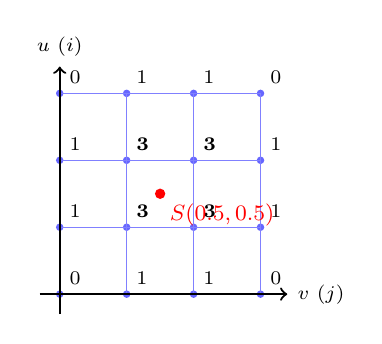
\begin{tikzpicture}[scale=0.85,every node/.style={font=\scriptsize}]
  \foreach \i in {0,1,2,3}{
    \foreach \j in {0,1,2,3}{
      \fill[blue!60] (\j,\i) circle (1.6pt);
    }
  }
  \foreach \i in {0,1,2,3}{
    \draw[blue!50,thin] (0,\i)--(1,\i)--(2,\i)--(3,\i);
  }
  \foreach \j in {0,1,2,3}{
    \draw[blue!50,thin] (\j,0)--(\j,1)--(\j,2)--(\j,3);
  }
  \node[above right] at (0,0) {$0$};
  \node[above right] at (1,0) {$1$};
  \node[above right] at (2,0) {$1$};
  \node[above right] at (3,0) {$0$};
  \node[above right] at (0,1) {$1$};
  \node[above right] at (1,1) {$\mathbf{3}$};
  \node[above right] at (2,1) {$\mathbf{3}$};
  \node[above right] at (3,1) {$1$};
  \node[above right] at (0,2) {$1$};
  \node[above right] at (1,2) {$\mathbf{3}$};
  \node[above right] at (2,2) {$\mathbf{3}$};
  \node[above right] at (3,2) {$1$};
  \node[above right] at (0,3) {$0$};
  \node[above right] at (1,3) {$1$};
  \node[above right] at (2,3) {$1$};
  \node[above right] at (3,3) {$0$};
  \fill[red] (1.5,1.5) circle (2.2pt);
  \node[red,below right] at (1.5,1.5) {\footnotesize $S(0.5,0.5)$};
  \draw[->,thick] (-0.3,0)--(3.4,0) node[right]{$v$ ($j$)};
  \draw[->,thick] (0,-0.3)--(0,3.4) node[above]{$u$ ($i$)};
\end{tikzpicture}
\end{center}
\textit{Nhìn từ trên xuống: số ghi là độ cao $z$ của $P_{ij}$. Chấm đỏ = hình chiếu của điểm cần tính.}

% ---------------------------------------------------------------------
\subsection*{6.6 Mẹo làm bài thi}

\begin{itemize}[leftmargin=*,nosep]
  \item \textbf{Ghi rõ hướng tham số:} viết ngay từ đầu trục nào là $u$ (hàng $i$), trục nào là $v$ (cột $j$) trước khi làm phép tính đầu tiên.
  \item \textbf{Cách hàng-trước (row-first) thường nhanh hơn} khi tính tay: tận dụng đối xứng giữa các hàng (vd.\ Hàng 0 đối xứng Hàng 3, Hàng 1 đối xứng Hàng 2) để bỏ qua phép tính trùng.
  \item \textbf{Luôn check chéo bằng Bernstein.} Tại $(0.5,0.5)$ trọng số bậc 3 là $(1,3,3,1)/8$, nên ma trận $4\times4$ là $\{1,3,9\}/64$ --- \emph{thuộc lòng bộ số này}.
  \item Kiểm tra tổng góc/cạnh/trong: $4{\cdot}1+8{\cdot}3+4{\cdot}9=64$.
  \item Với $(u,v)$ khác, tính $B_i^3(u)$ và $B_j^3(v)$ riêng, rồi nhân ngoài (outer product) thành ma trận $4\times4$.
  \item $S(u,v)$ ở 4 góc bằng đúng 4 control point góc: $S(0,0)=P_{00}$,\dots --- dùng để kiểm tra nhanh.
\end{itemize}

\end{paracol}
